% CVPR 2025 Paper Template; see https://github.com/cvpr-org/author-kit

\documentclass[10pt,twocolumn,letterpaper]{article}

%%%%%%%%% PAPER TYPE  - PLEASE UPDATE FOR FINAL VERSION
\usepackage{cvpr}              % To produce the CAMERA-READY version
% \usepackage[review]{cvpr}      % To produce the REVIEW version
% \usepackage[pagenumbers]{cvpr} % To force page numbers, e.g. for an arXiv version

% Import additional packages in the preamble file, before hyperref
%
% --- inline annotations
%
\newcommand{\red}[1]{{\color{red}#1}}
\newcommand{\todo}[1]{{\color{red}#1}}
\newcommand{\TODO}[1]{\textbf{\color{red}[TODO: #1]}}
% --- disable by uncommenting  
% \renewcommand{\TODO}[1]{}
% \renewcommand{\todo}[1]{#1}



% It is strongly recommended to use hyperref, especially for the review version.
% hyperref with option pagebackref eases the reviewers' job.
% Please disable hyperref *only* if you encounter grave issues, 
% e.g. with the file validation for the camera-ready version.
%
% If you comment hyperref and then uncomment it, you should delete *.aux before re-running LaTeX.
% (Or just hit 'q' on the first LaTeX run, let it finish, and you should be clear).
\definecolor{cvprblue}{rgb}{0.21,0.49,0.74}
\usepackage[pagebackref,breaklinks,colorlinks,allcolors=cvprblue]{hyperref}

\usepackage{algorithm,algpseudocode,float}
\usepackage{lipsum}
\usepackage{longtable}
\usepackage{multirow}
\usepackage{graphicx}

\makeatletter
\newenvironment{breakablealgorithm}
  {% \begin{breakablealgorithm}
   \begin{center}
     \refstepcounter{algorithm}% New algorithm
     \hrule height.8pt depth0pt \kern2pt% \@fs@pre for \@fs@ruled
     \renewcommand{\caption}[2][\relax]{% Make a new \caption
       {\raggedright\textbf{\ALG@name~\thealgorithm} ##2\par}%
       \ifx\relax##1\relax % #1 is \relax
         \addcontentsline{loa}{algorithm}{\protect\numberline{\thealgorithm}##2}%
       \else % #1 is not \relax
         \addcontentsline{loa}{algorithm}{\protect\numberline{\thealgorithm}##1}%
       \fi
       \kern2pt\hrule\kern2pt
     }
  }{% \end{breakablealgorithm}
     \kern2pt\hrule\relax% \@fs@post for \@fs@ruled
   \end{center}
  }
\makeatother

%%%%%%%%% PAPER ID  - PLEASE UPDATE
\def\paperID{*****} % *** Enter the Paper ID here
\def\confName{CVPR}
\def\confYear{2025}

\title{Exploration of Adversarial Training}

%%%%%%%%% AUTHORS - PLEASE UPDATE
\author{Jiarui HE\\
College of Education Sciences \\
The Hong Kong University of Science and Technology (Guangzhou) \\
{\tt\small jhe218@connect.hkust-gz.edu.cn}
}

\begin{document}
\maketitle

\begin{abstract}
Adversarial examples—small, intentionally crafted perturbations to input data—pose a critical threat to the reliability of modern machine learning models. In this report, we first review the theoretical foundations of adversarial robustness, formalizing the min-max optimization objective that underlies adversarial training. We then survey prominent attack and defense algorithms, including Projected Gradient Descent (PGD), and the FreeLB framework. To assess practical performance, we conduct an empirical study on a lightweight seven-layer convolutional network, comparing standard training against PGD- and FreeLB-based adversarial training under varying perturbation intensities. Our results show that multi-step adversarial training increases robust accuracy from roughly 56\% to over 95\% under strong PGD attacks, while incurring a modest decrease in clean-data accuracy and a significant rise in training time. Then, we discuss the principal challenges—namely, the robustness-accuracy trade-off, high computational cost. Finally, we discuess the further application of adversarial training and related concepts, including GANs and Adversarial Explainability.
\end{abstract}

\section{Introduction}

Adversarial training plays a fundamental role in artificial intelligence applications, particularly in the context of neural networks. By incorporating adversarial examples into the training process, models can achieve enhanced robustness against perturbed inputs, including those specifically crafted to deceive the network. Consequently, adversarial training bolsters the security and reliability of AI systems. Moreover, related methodologies have catalyzed significant advancements in generative artificial intelligence.

Section 2 reviews several widely adopted adversarial training algorithms. Section 3 presents a case study illustrating the impact of adversarial training on model performance. Section 4 examines the challenges and limitations inherent to adversarial training. Finally, Section 5 explores additional applications and future directions for this paradigm.

\section{Training Algorithms}
Let $\theta$ be the parameters of models, $f_\theta(\cdot)$ be the model, $\epsilon$ be the range of perturb of attack sample and $L$ be the loss function.

Then the target of adversarial training can be

\begin{equation}
\theta^*=\arg\min_\theta\left\{
  \mathbb{E}_{(\mathbf{x}, \mathbf{y})\in \mathcal{D}}
  \left[
      \max_{\lVert\mathbf{\delta}\rVert\leq \epsilon}
          \left\{L(f_\theta(\mathbf{x}+\delta), y)\right\}
  \right]
\right\}
\tag{2:1}
\label{formula:adversarial_target}
\end{equation}

Adversarial training plays a fundamental role in artificial intelligence applications, particularly in the context of neural networks. By incorporating adversarial examples into the training process, models can achieve enhanced robustness against perturbed inputs, including those specifically crafted to deceive the network. Consequently, adversarial training bolsters the security and reliability of AI systems. Moreover, related methodologies have catalyzed significant advancements in generative artificial intelligence.

Section 2 and Section 3 reviews several widely adopted adversarial training algorithms. Section 4 presents a case study illustrating the impact of adversarial training on model performance. Section 5 examines the challenges and limitations inherent to adversarial training. Finally, Section 6 explores additional applications and future directions for this paradigm.

\section{Adversarial Training Objective}
Let $\theta$ denote the model parameters, $f_{\theta}(\cdot)$ the model mapping, $\epsilon$ the maximum allowable perturbation magnitude, and $L(\cdot,\cdot)$ the loss function. The objective of adversarial training can then be formulated as:

\begin{equation}
\theta^{*} = \arg\min_{\theta} ; \mathbb{E}{(\mathbf{x},\mathbf{y}) \sim \mathcal{D}} \Biggl[\underbrace{\max_{{\lVert \mathbf{\delta} \rVert \le \epsilon}} L\bigl(f_{\theta}(\mathbf{x} + \mathbf{\delta}), \mathbf{y}\bigr)}_{\text{worst-case loss}}\Biggr]
\label{eq:adv_training_objective}
\end{equation}

Here, the inner maximization identifies the most adversarial perturbation $\mathbf{\delta}$ within the $\epsilon$-ball around the input $\mathbf{x}$, while the outer minimization optimizes the model parameters to minimize the expected worst-case loss over the data distribution $\mathcal{D}$.

\section{Adversarial Training Algorithms}
Several algorithms have been proposed to approximate the inner maximization in Equation~\eqref{eq:adv_training_objective}. Among these, the projected gradient descent (PGD) method is one of the most classical and widely used approaches. Subsequent techniques often build upon PGD, introducing modifications to improve efficiency, convergence, or transferability.

\subsection{Projected Gradient Descent (PGD)}
The PGD attack iteratively constructs adversarial examples by ascending the gradient of the loss with respect to the input. At each step, the perturbation is updated and then projected back onto the allowable perturbation set:

$$
\begin{aligned}
\mathbf{\delta}_{0} &= \mathbf{0}, \\
\mathbf{\delta}_{t+1} &= \Pi_{{\lVert \mathbf{\delta_t} \rVert \le \epsilon}} \Bigl(\mathbf{\delta}_{t} + \alpha \cdot \mathrm{sign}\bigl(\nabla_{\mathbf{x}} L(f_{\theta}(\mathbf{x} + \mathbf{\delta}_{t}), \mathbf{y})\bigr)\Bigr),
\end{aligned}
$$

where:

$\alpha$ is the step size hyperparameter, and $k$ denotes the total number of iterations (denoted as PGD-$k$).

$\Pi$ represents the projection operator onto the $\ell_{p}$-ball of radius $\epsilon$, commonly using $p=2$ or $p=\infty$.

After $k$ iterations, the adversarial example is given by $\mathbf{x}^{\mathrm{adv}} = \mathbf{x} + \mathbf{\delta}_{k}$. Incorporating these examples into the training process yields the PGD adversarial training algorithm

\begin{breakablealgorithm}
\caption{PGD training}
\begin{algorithmic}[1] %每行显示行号
  \Require training set $\mathcal{D}$, learning rate $\tau$, training epochs $N$, hyperparameters $\alpha, \epsilon, k$, model $f_\theta$ and loss function $L$
  \State Initialize model parameters $\theta$

  \For {$n=1$ to $N$}
    \State {divide $\mathcal{D}$ into list of mini-batches $\mathcal{C}=\{(\mathrm{X}, \mathbf{y})\}$}
    \For {$(\mathrm{X}, \mathbf{y})\in \mathcal{C}$} 
      \State {$\delta\leftarrow$ zero matrix with shape of $X$}
      \For {$t\leftarrow 1$ to $k$}
        \State {execute backpropagation}
        \State $g_a\leftarrow \nabla_{\mathrm{X}+\delta}(L(f_{\theta}(\mathrm{X}+\delta), \mathbf{y}))$
        \State $\delta\leftarrow \mathrm{clamp}(\delta + \frac{\alpha}{\left\lVert g_a \right\rVert}g_a, -\epsilon, \epsilon)$
      \EndFor
      \State $g_\theta\leftarrow \nabla_{\theta}(L(f_{\theta}(\mathrm{X}+\delta), \mathbf{y}))$
      \State $\theta \leftarrow \theta - \tau g_\theta$
    \EndFor
  \EndFor
\end{algorithmic}
\end{breakablealgorithm}

Overall, the times of forward propagation and backpropagation of this algorithm are both $\Theta (NMk)$, where $M$ is the number of mini-batches

\subsection{You can Only Propagate Once (YOPO)}

The YOPO algorithm aims to improve computational efficiency during adversarial training by reducing the number of full backpropagation operations. Leveraging insights from the Pontryagin Maximum Principle (PMP), YOPO posits that the model's first layer is primarily responsible for responding to adversarial perturbations. Based on this assumption, the algorithm reuses gradients for all layers except the first across multiple inner-loop iterations.

In this framework, each mini-batch is processed through a two-level loop structure defined by hyperparameters $m$ and $n$. The outer loop executes full backpropagation once to compute gradients for all layers except the first. Within the inner loop, adversarial perturbations are iteratively updated using gradients computed only for the first layer. The configuration is denoted as YOPO-$m$-$n$.

The pseudocode for this method is presented below:

\begin{breakablealgorithm}
\caption{YOPO training}
\begin{algorithmic}[1]
  \Require training set $\mathcal{D}$, learning rate $\tau$, training epochs $N$, hyperparameters $\alpha, \epsilon, m, n$, model $f_\theta$ and loss function $L$ 
  \State divide the model parameters $\theta$ into first layer $\theta_0$ and the other layers $\theta'$
  \For {$i\leftarrow 1$ to $N$}
    \State {divide $\mathcal{D}$ into list of mini-batches $\mathcal{C}=\{(\mathrm{X}, \mathbf{y})\}$}
    \For {$(\mathrm{X}, \mathbf{y})\in \mathcal{C}$}
      \State $\delta_{0, n}\leftarrow \text{zero matrix with shape of } \mathrm{X}$
      \State $g_\theta\leftarrow \text{zero matrix with shape of } \mathrm{\theta}$
      \For {$j=1$ to $m$}
        \State execute entire backpropagation
        \State $\delta_{j,0}\leftarrow \delta_{j-1,n}$
        \State {$p\leftarrow \nabla_{f_{\theta_0}(\mathrm{X}+\delta_{j,0})}\left(
          L(f_\theta(\mathrm{X}+\delta_{j,0}), \mathbf{y})
        \right)$}
        \For {$k=1$ to $n$}
          \State $g_a\leftarrow
            p\cdot \nabla_{\mathrm{X}+\delta}(f_{\theta_0}(\mathrm{X}+\delta_{j,k-1}))$
          \State $\delta_{j,k}\leftarrow \mathrm{clamp}\left(\delta_{j,k-1}+\frac{\alpha\cdot g_a}{\left\lVert g_a \right\rVert}, -\epsilon, \epsilon\right)$
        \EndFor
        \State $g_\theta\leftarrow g_\theta + \nabla_{\theta}(L(f_{\theta}(\mathrm{X}+\delta_{j,n}), \mathbf{y}))$
        \Comment this gradient can be calculated in backpropagation
      \EndFor
      \State $\theta\leftarrow \theta-\tau\cdot g_\theta$
    \EndFor
  \EndFor
\end{algorithmic}
\end{breakablealgorithm}

In this scheme, full backpropagation is performed only $\mathcal{O}(m)$ times per mini-batch, whereas adversarial example updates occur $\mathcal{O}(mn)$ times. According to Zhang et al.~\cite{zhang2019propagateonceacceleratingadversarial}, if $m \times n$ slightly exceeds $k$, YOPO-$m$-$n$ can achieve comparable performance to PGD-$k$ with significantly reduced computational cost.

Nonetheless, other analyses~\cite{zhu2020freelbenhancedadversarialtraining} suggest that the PMP-based assumptions underlying YOPO may not hold in models utilizing ReLU activation functions.

\subsection{Free Large Batch Adversarial Attack (FreeLB)}

ifferent from PGD, which performs $k$ iterations to generate an adversarial example and uses only the final perturbed sample to update the model, FreeLB aggregates the gradient contributions from all intermediate perturbations by averaging them. This strategy leverages the full spectrum of adversarial information encountered during the iterative process.

FreeLB can be viewed as a special case of YOPO when the number of inner iterations $m$ is set to 1. Unlike YOPO, however, FreeLB is also applicable to models employing ReLU activations, which are common in modern architectures.

In contrast to PGD, which first performs multiple inner maximizations to generate a strong adversarial example and then applies a single gradient descent update on the model parameters, FreeLB interleaves the two processes. Specifically, it performs model updates after each inner-loop maximization step. This interleaved optimization approach has been shown to improve both model robustness and training efficiency~\cite{zhu2020freelbenhancedadversarialtraining}.

The pseudocode for the FreeLB training procedure is as follows:

\begin{breakablealgorithm}
\caption{FreeLB training}
\begin{algorithmic}[1]
  \Require training set $\mathcal{D}$, learning rate $\tau$, training epochs $N$, hyperparameters $\alpha, \epsilon, k$, model $f_\theta$ and loss function $L$ .
  \For {$i\leftarrow 1$ to $N$}
    \State {divide $\mathcal{D}$ into list of mini-batches $\mathcal{C}=\{(\mathrm{X}, \mathbf{y})\}$}
    \For {$(\mathrm{X}, \mathbf{y})\in \mathcal{C}$}
      \State $\delta_0\leftarrow \textbf{random}\text{ matrix with shape of } \mathrm{X}$
      \State $g_\theta\leftarrow \text{zero matrix with shape of } \theta$
      \For {$i\leftarrow 1$ to $k$}
        \State {execute backpropagation}
        \State $g_\theta\leftarrow g_\theta + \frac{1}{k}\nabla_{\theta}(L(f_\theta(\mathrm{X}+\delta_{i-1}), \mathbf{y}))$
        \State $g_a\leftarrow \nabla_{\mathrm{X}+\delta}(L(f_\theta(\mathrm{X}+\delta_{i-1}), \mathbf{y}))$
        \State $\delta_i\leftarrow \mathrm{clamp}\left(\delta_{i-1}+\frac{\alpha}{\left\lVert g_a \right\rVert}g_a, -\epsilon, \epsilon\right)$
      \EndFor
      \State {$\theta\leftarrow\theta-\tau g_\theta$}
    \EndFor
  \EndFor
\end{algorithmic}
\end{breakablealgorithm}

However, it is important to note that performing full backpropagation and accumulating gradients at each inner-loop iteration incurs higher computational cost. This computational overhead is empirically demonstrated in Table~\ref{table:instance_training-result}.

\subsection{SMoothness-inducing Adversarial Regularization (SMART)}

Unlike traditional adversarial training approaches that directly aim to optimize the objective defined in Equation~\ref{eq:adv_training_objective}, this algorithm treats adversarial perturbations as a form of regularization. Specifically, it encourages the model to produce consistent predictions for inputs within a small neighborhood in the input space. This regularization-based adversarial training paradigm has been shown to be particularly effective for fine-tuning pre-trained language models in natural language processing tasks~\cite{Jiang_2020}.

The corresponding optimization objective is defined as follows:

\begin{equation}
\theta^* = \arg\min_\theta\left\{\mathcal{L}(\theta) + \lambda \mathcal{R}(\theta)\right\}
\tag{2:4:1}
\label{formula:adversarial_target2}
\end{equation}

Here, $\mathcal{L}(\theta)$ denotes the empirical risk over the training dataset, $\lambda > 0$ is a hyperparameter balancing the two terms, and $\mathcal{R}(\theta)$ is a smoothness-inducing adversarial regularization term. The detailed formulations are given by:

$$
\begin{aligned}
  &\mathcal{L}(\theta)=\frac{1}{n}\sum_{(\mathbf{x}, \mathbf{y})\in\mathcal{D}} L(f_\theta(\mathbf{x}), \mathbf{y}) \\
  &\mathcal{R}(\theta)=\frac{1}{n}\sum_{(\mathbf{x}, \mathbf{y})\in\mathcal{D}} \max_{\left\Vert \tilde{\mathbf{x}}-\mathbf{x}\right\Vert\leq \epsilon}\left\{l\left(f_\theta(\tilde{\mathbf{x}}), f_\theta(\mathbf{x})\right)\right\}
\end{aligned}
$$

The divergence measure $l(a, b)$ used in $\mathcal{R}(\theta)$ is the symmetric Kullback-Leibler (KL) divergence defined as:

$$
\begin{aligned}
l(f, g)&=\mathrm{KL}(f\Vert g) + \mathrm{KL}(g\Vert f) \\
&=\sum_{x\in \mathcal{X}} f(x)\log\frac{f(x)}{g(x)} + g(x)\log\frac{g(x)}{f(x)} \\
&=\sum_{x\in \mathcal{X}} (f(x) - g(x))\log\frac{f(x)}{g(x)}
\end{aligned}
$$

To optimize the objective in Equation~\ref{formula:adversarial_target2}, the algorithm adopts a Bregman proximal point optimization framework. The core component of this framework is the Bregman divergence, defined over dataset $\mathcal{D}$ as:

$$
\mathrm{Breg}_\mathcal{D}(\theta_1, \theta_2)=\frac{1}{\left\vert\mathcal{D}\right\vert}
  \sum_{(\mathbf{x}, \mathbf{y})\in\mathcal{D}}l\left(f_{\theta_1}(\mathbf{x}), f_{\theta_2}(\mathbf{x})\right)
$$

For each mini-batch, this divergence serves as a surrogate loss to guide the generation of adversarial perturbations. More specifically, the gradient of the perturbation $\delta$ for a mini-batch $\mathcal{D}$ is computed as follows:

$$
g_\theta(\mathcal{D}, \delta)=
\begin{bmatrix}
  \nabla_{\delta_1}l(f_\theta(\mathbf{x}_1), f_\theta(\mathbf{x}_1+\delta_1)) \\
  \nabla_{\delta_2}l(f_\theta(\mathbf{x}_2), f_\theta(\mathbf{x}_2+\delta_2)) \\
  \vdots \\
  \nabla_{\delta_{|\mathcal{D}|}}l\left(f_\theta\left(\mathbf{x}_{|\mathcal{D}|}\right), f_\theta\left(\mathbf{x}_{|\mathcal{D}|}+\delta_{|\mathcal{D}|}\right)\right)
\end{bmatrix}
$$

To further enhance optimization stability and convergence, momentum and the Adam update rule are applied throughout the training process. The pseudocode outlining this algorithm will be presented below.

\begin{breakablealgorithm}
\caption{SMART training}
\begin{algorithmic}[1]
  \Require number of iteration of attack sample $k$, dataset $\mathcal{D}$, parameters of pre-trained model $\theta_0$ , number of epochs $N$, learning rate $\tau$, hyperparameters for iteration of attack sample $\alpha, \epsilon$, momentum parameter $\beta$

  \State $\tilde{\theta_1}\leftarrow\theta_0$ 
  \For {$t\leftarrow 1$ to $N$}
    \State $\overline{\theta}\leftarrow \theta_{t-1}$
    \State {divide $\mathcal{D}$ into mini-batches $\mathcal{C}$}
    \For {$(\mathrm{X}, \mathbf{y})\in \mathcal{C}$}
      \State initialize $\delta$ with guassian distribution
      \State $\forall \delta _i\sim N(0,\sigma^2I)$
      \For {$i=1$ to $k$}
        \State $g_i\leftarrow \frac{g_{\overline{\theta}}\left((\mathrm{X},\mathbf{y}), \delta\right)}{\left\Vert g_{\overline{\theta}}((\mathrm{X},\mathbf{y}), \delta) \right\Vert}$
        \State $\delta\leftarrow \mathrm{clamp}(\delta + \alpha g_i, -\epsilon, \epsilon)$
      \EndFor
      \State $\overline{\theta}\leftarrow \mathrm{Adam}\left(\overline{\theta}, (\mathrm{X}+\delta, \mathbf{y})\right)$
    \EndFor
    \State $\theta_t\leftarrow \overline{\theta}$
    \State $\tilde{\theta}_{t+1}\leftarrow (1-\beta)\overline{\theta}+\beta\tilde{\theta}_t$
  \EndFor
  \State the output is $\theta_N$
\end{algorithmic}
\end{breakablealgorithm}

\section{An Instance of Adversarial Training}

To provide a concrete illustration of adversarial training and facilitate analysis of its characteristics and effectiveness, we conducted empirical experiments using both PGD and FreeLB algorithms.

The experiments were implemented using the \texttt{torch} library. The dataset utilized was MNIST, a widely adopted benchmark for image classification tasks. The computational environment comprised an NVIDIA RTX 2080Ti GPU (22GB VRAM) and an Intel Core i9-13900K CPU.

For all experiments, the learning rate was set to $1 \times 10^{-4}$, and the number of training epochs was fixed at 50. The Adam optimizer was employed for parameter updates.

The model used was a lightweight convolutional neural network, whose architecture is summarized in Table~\ref{table:instance_model-arch}:

\begin{table}[H]
  \centering
  \caption{Architecture of Model}
  \label{table:instance_model-arch}
  \begin{tabular}{cl}
    \textbf{Structure} & \textbf{Parameters} \\
    \hline
    \multirow{4}*{Conv2d} & $\texttt{filter}=32$ \\
    ~ & $\texttt{kernel}=5$ \\
    ~ & $\texttt{padding}=2$ \\
    ~ & $\texttt{bias}=\texttt{True}$ \\
    \hline
    \multirow{2}*{MaxPool2d} & $\texttt{kernel}=2$ \\
    ~ & $\texttt{stride}=2$ \\
    \hline
    \multirow{4}*{Conv2d} & $\texttt{filter}=32$ \\
    ~ & $\texttt{kernel}=5$ \\
    ~ & $\texttt{padding}=2$ \\
    ~ & $\texttt{bias}=\texttt{True}$ \\
    \hline
    \multirow{2}*{MaxPool2d} & $\texttt{kernel}=2$ \\
    ~ & $\texttt{stride}=2$ \\
    \hline
    \multirow{2}*{Linear} & $\texttt{input}=7\times 7\times 64$ \\
    ~ & $\texttt{output}=1024$ \\
    \hline
    \multirow{2}*{Linear} & $\texttt{input}=1024$ \\
    ~ & $\texttt{output}=10$ \\
  \end{tabular}
\end{table}

And here is the training result, where std represents the instance of training on original samples:

\begin{table}[H]
  \caption{Result of Adversarial Training}
  \label{table:instance_training-result}
  \begin{tabular}{lcccc}
    \multirow{2}*{\textbf{Training}} & \multicolumn{3}{c}{\textbf{Testing}} & \multirow{2}*{\textbf{Time}(min)} \\
    ~ & std & PGD-10 & PGD-40 & ~ \\
    \hline
    std & 98.46\% & 89.53\% & 56.40\% & 7.17 \\
    PGD-10 & 97.36\% & 98.00\% & 90.03\% & 12.87  \\
    PGD-40 & 88.36\% & 98.31\% & 95.81\% & 30.58 \\
    FreeLB-10 & 98.34\% & 97.79\% & 87.50\% & 20.18 \\
    FreeLB-40 & 94.96\% & 98.29\% & 94.90\% & 61.38 
  \end{tabular}
\end{table}

The record of training process is also provided :

\begin{figure}[H]
\centering
\caption{Test With Original Samples}
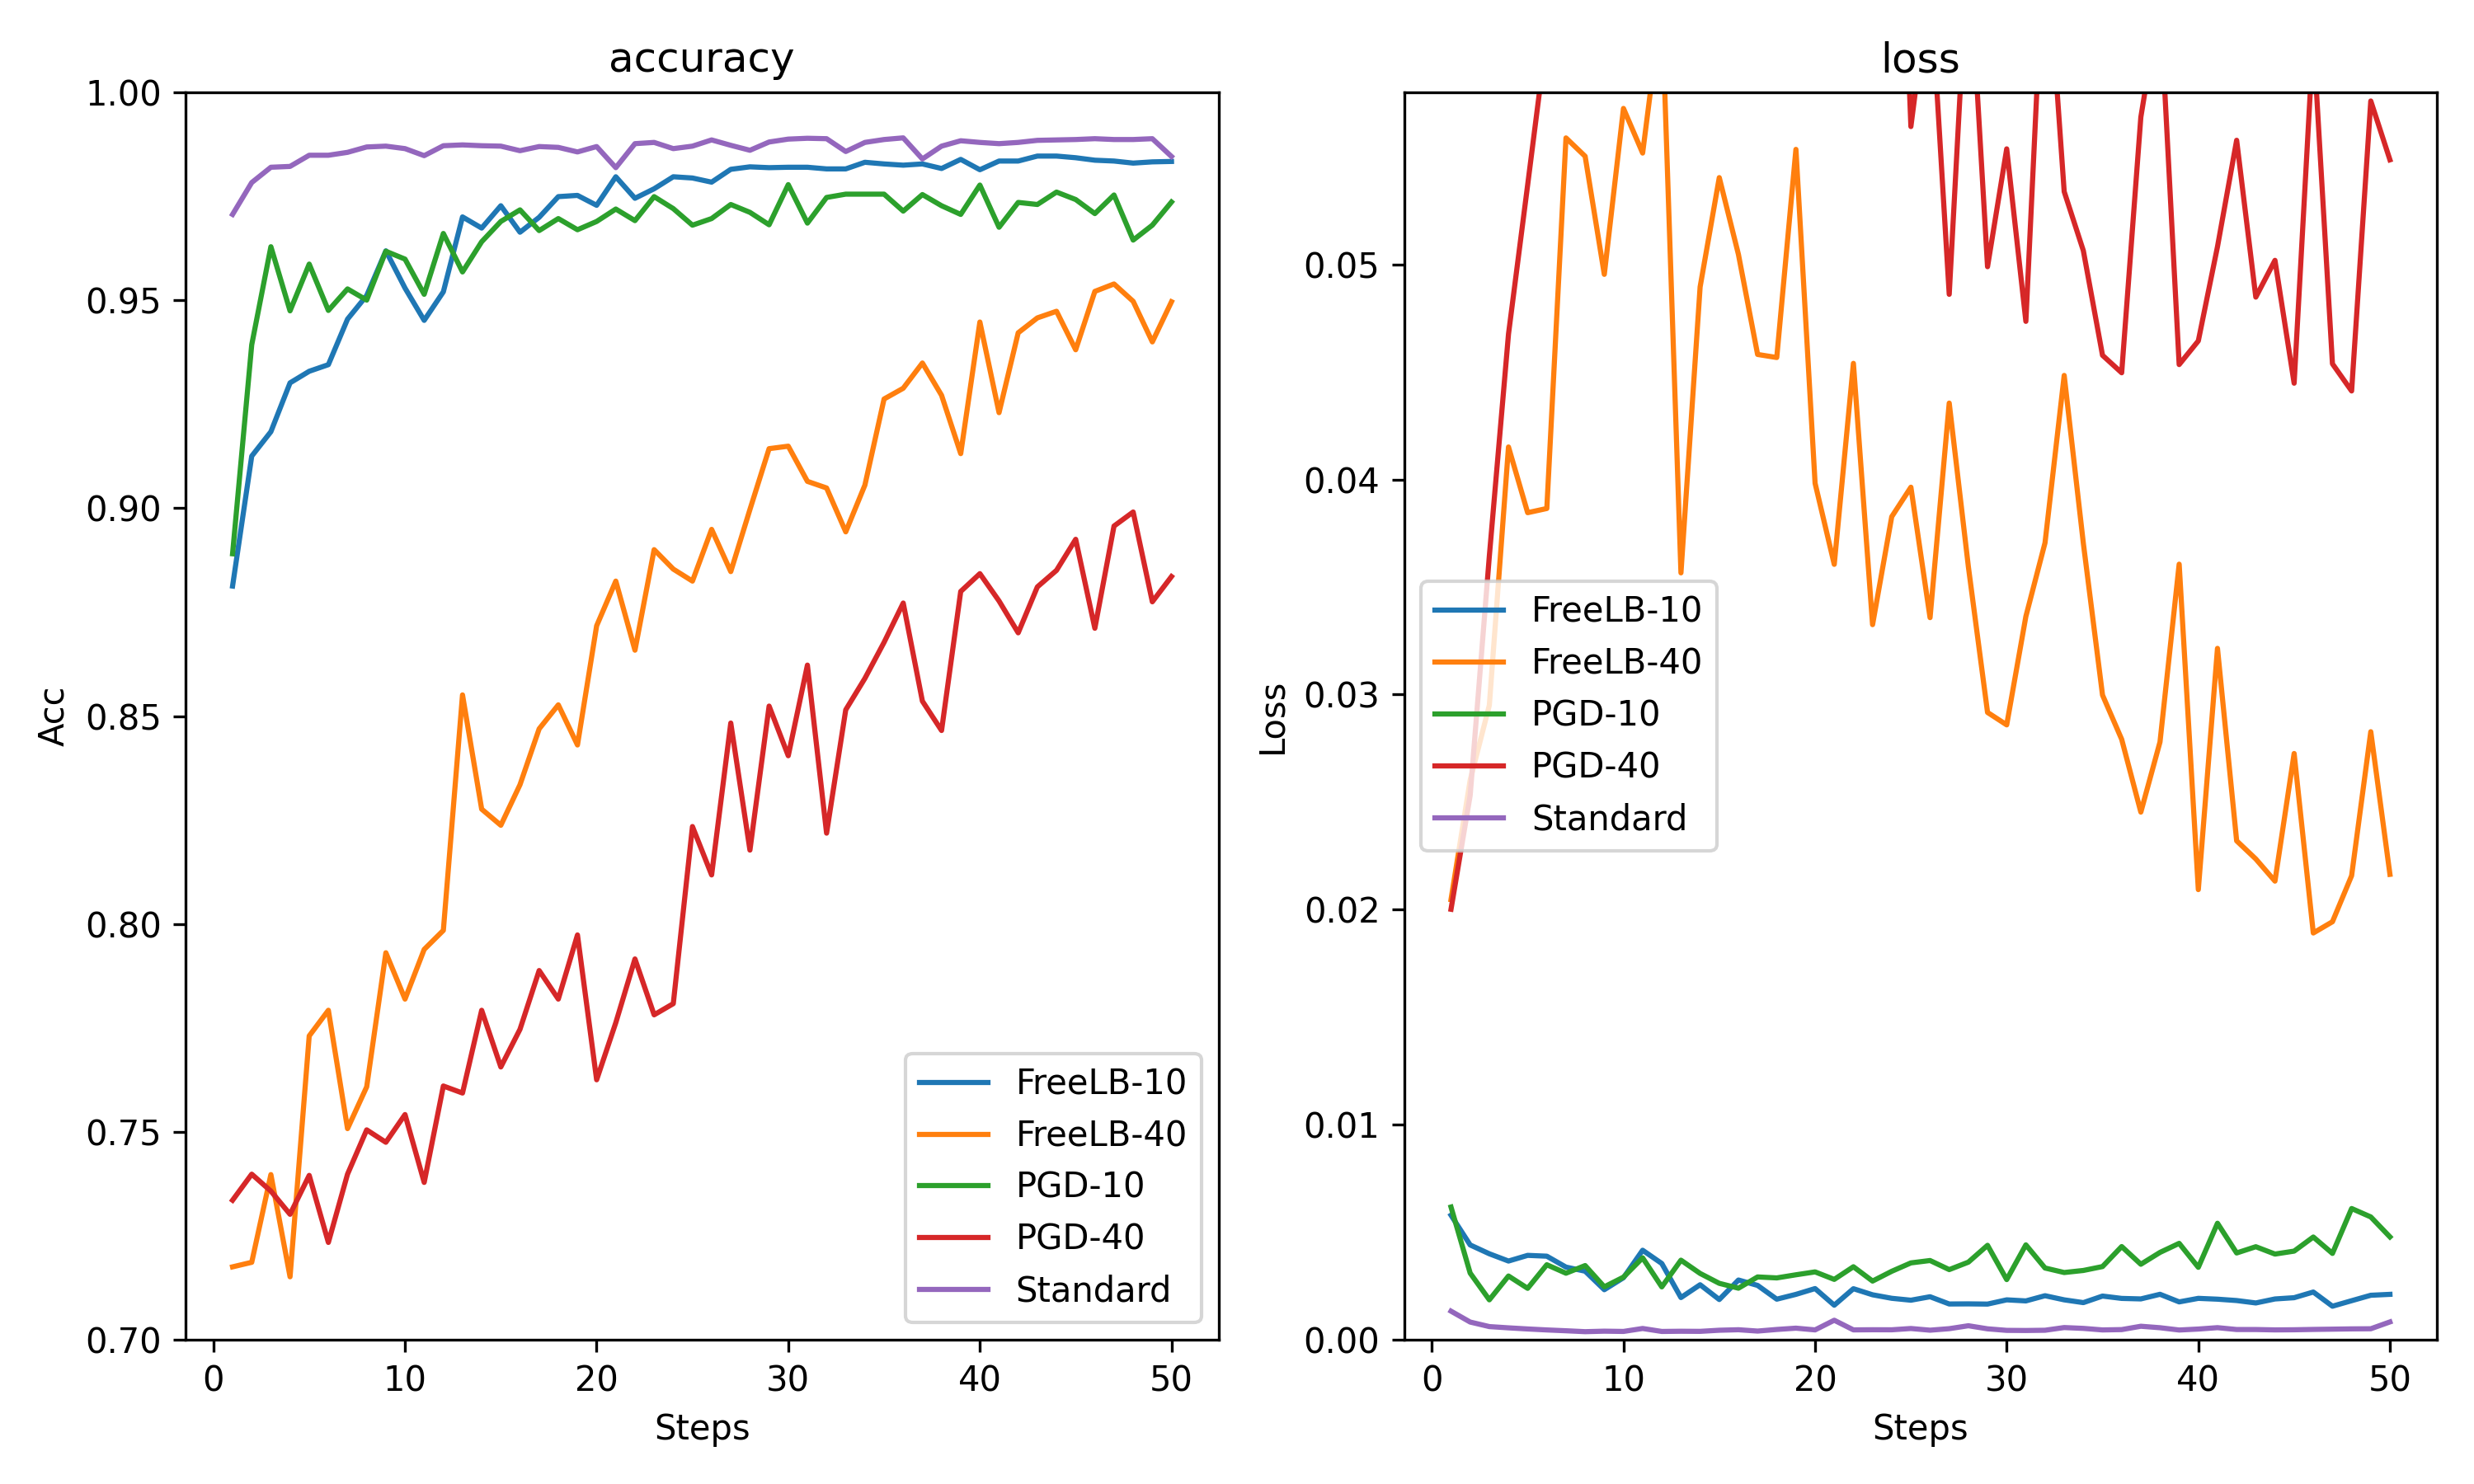
\includegraphics[width=0.45\textwidth]{figures/plot-Original.png}
\end{figure}

\begin{figure}[H]
\centering
\caption{Test With PGD-10}
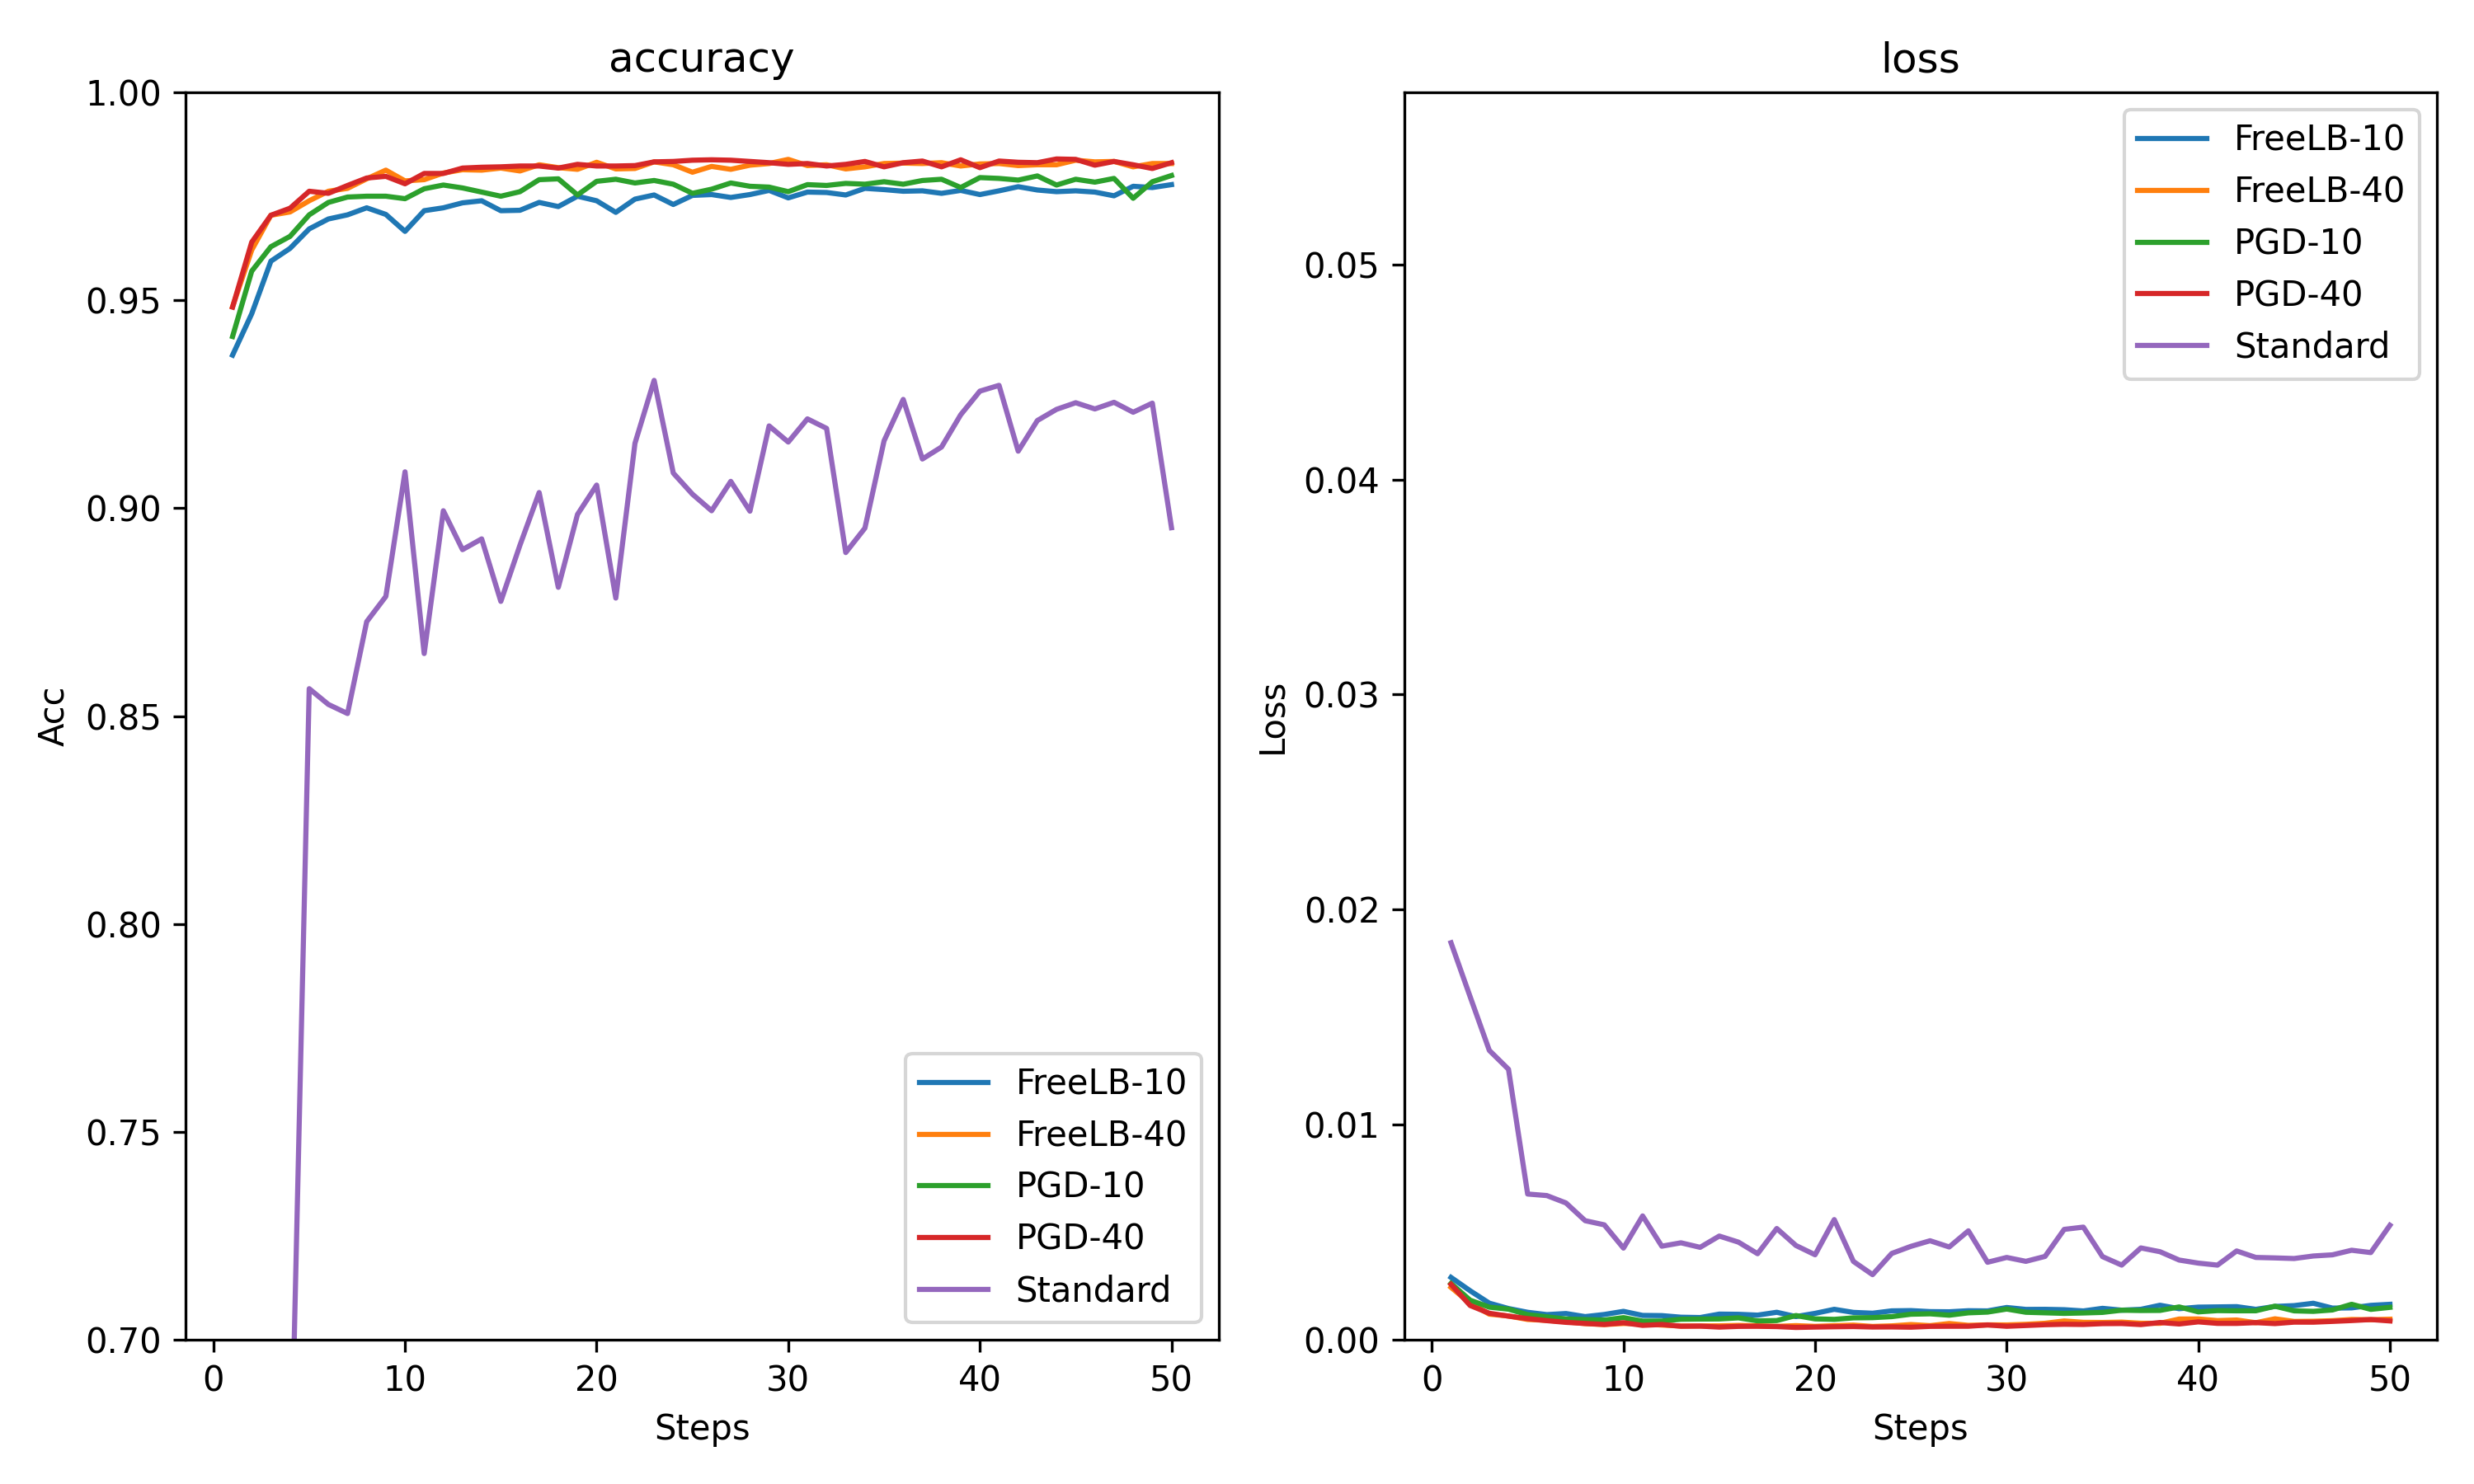
\includegraphics[width=0.45\textwidth]{figures/plot-PGD-10 Attack.png}
\end{figure}

\begin{figure}[H]
\centering
\caption{Test With PGD-40}
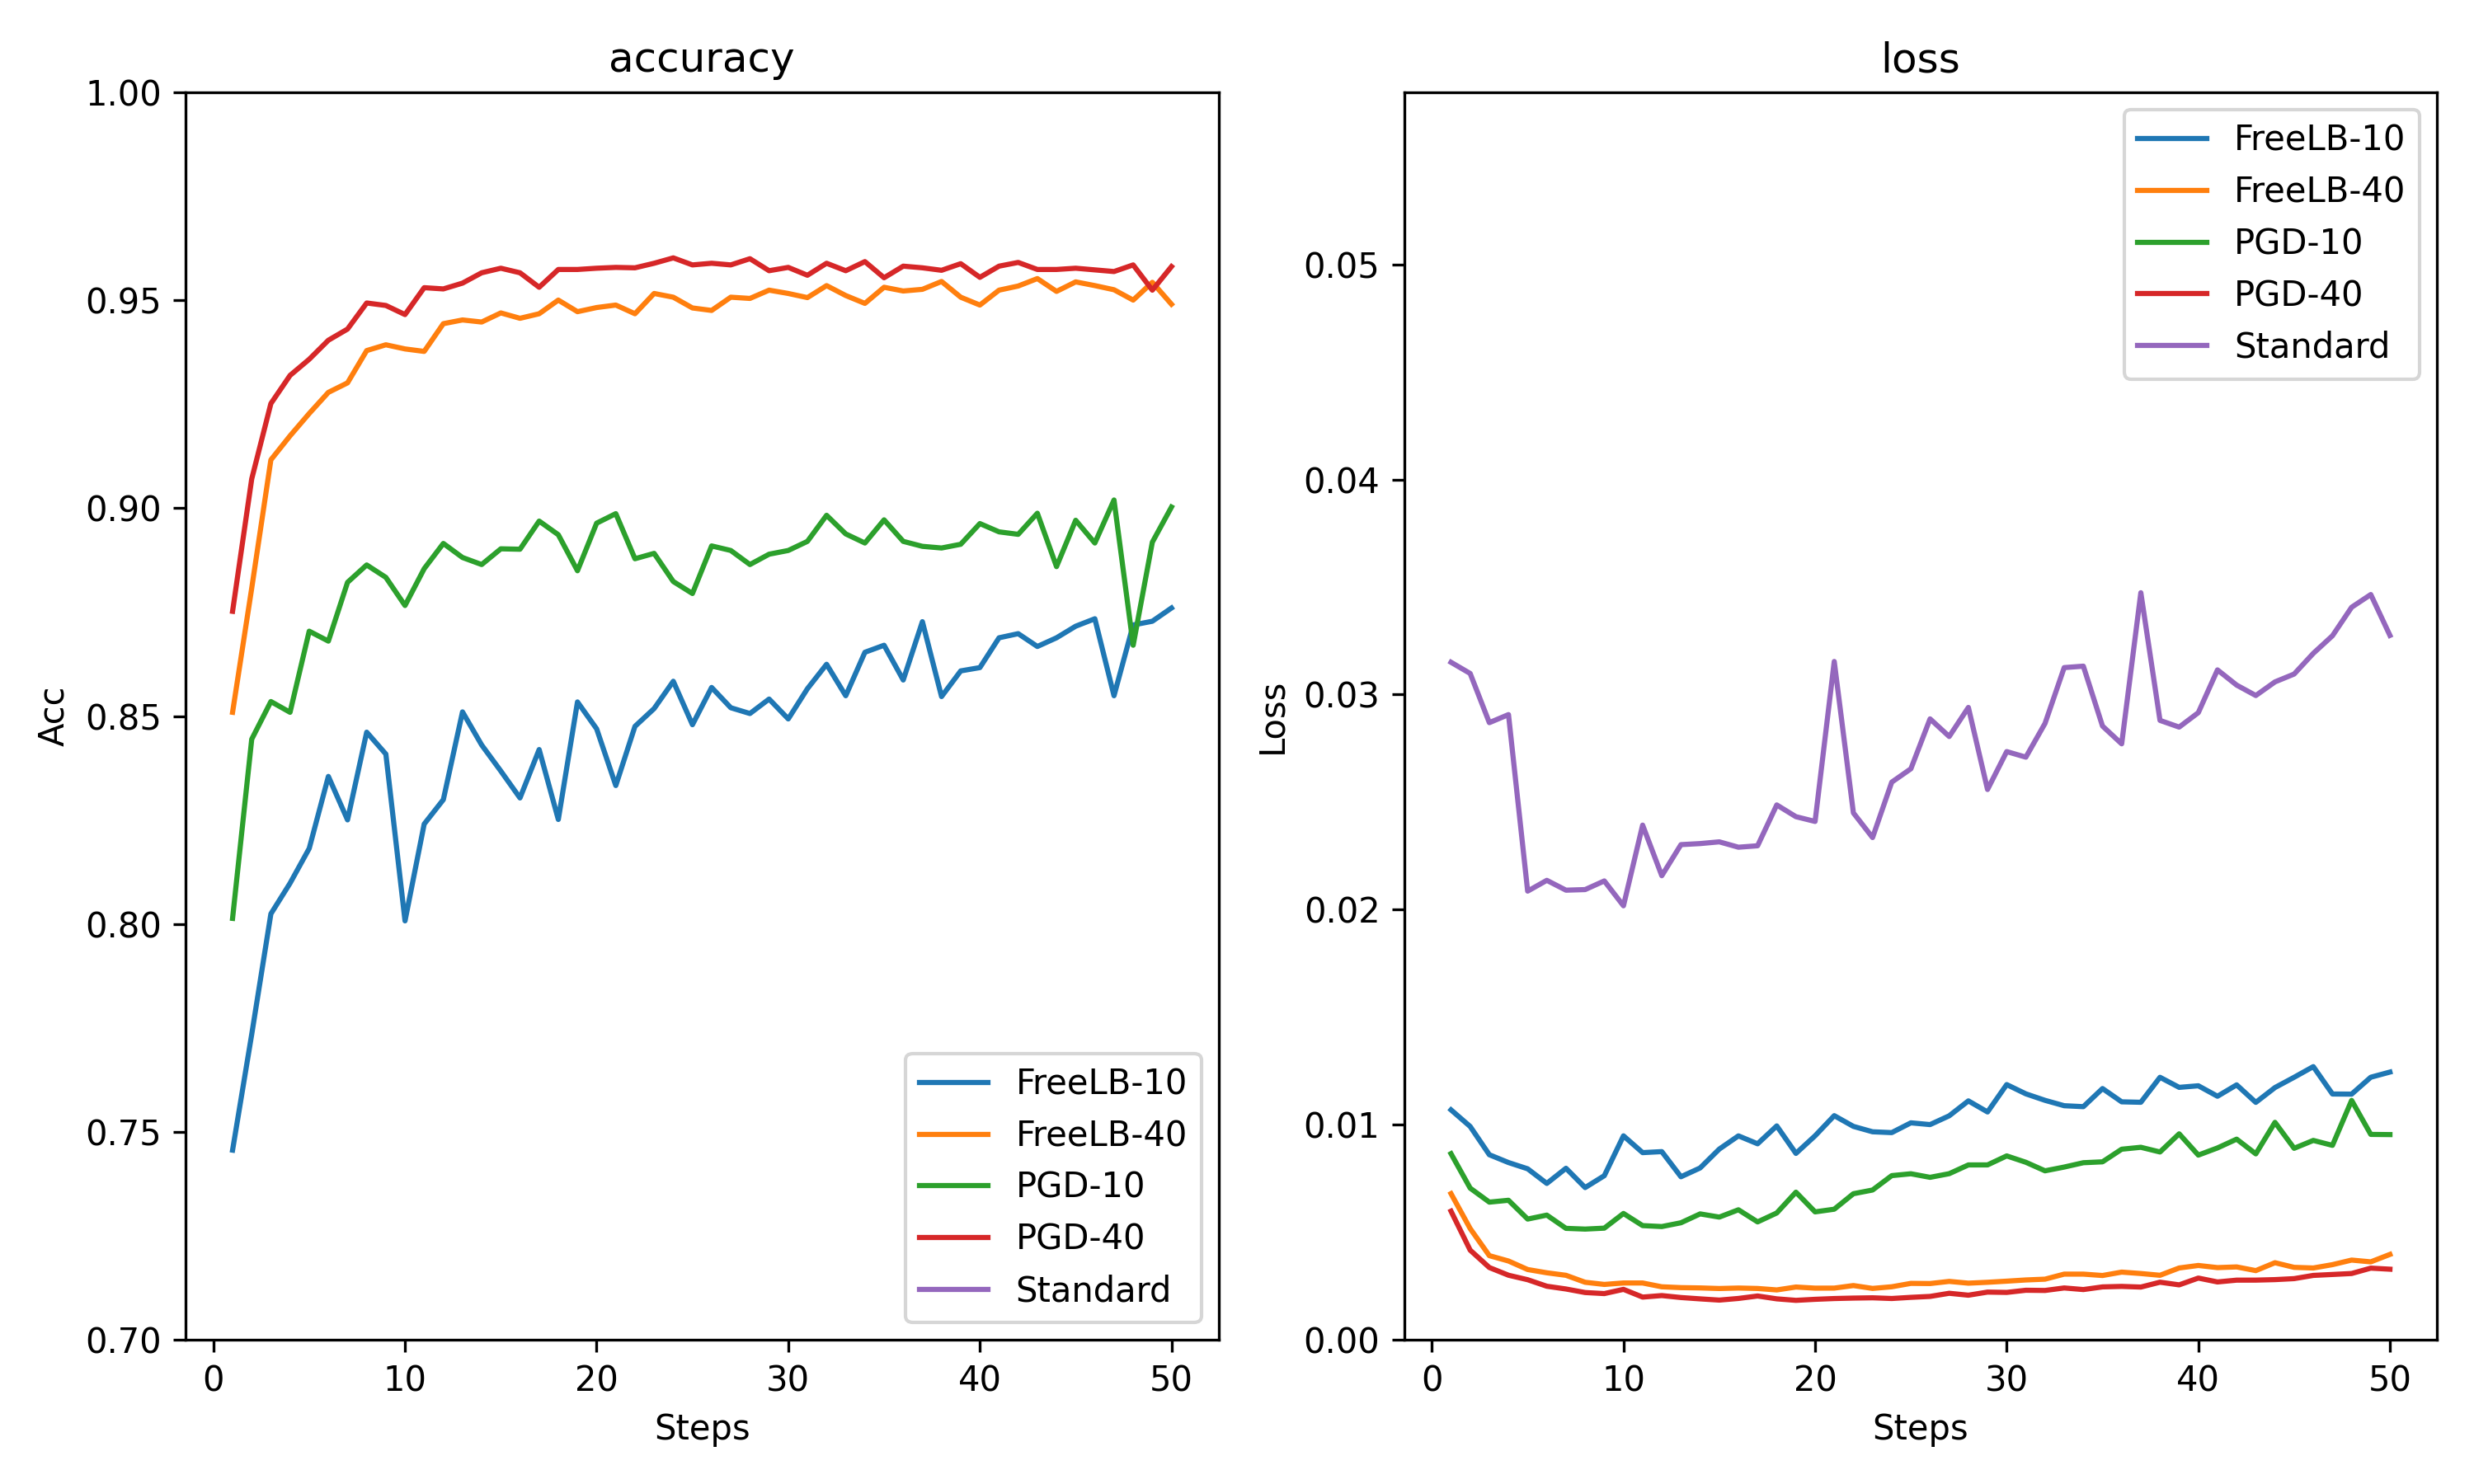
\includegraphics[width=0.45\textwidth]{figures/plot-PGD-40 Attack.png}
\end{figure}

\begin{figure}[H]
\centering
\caption{On Training set}
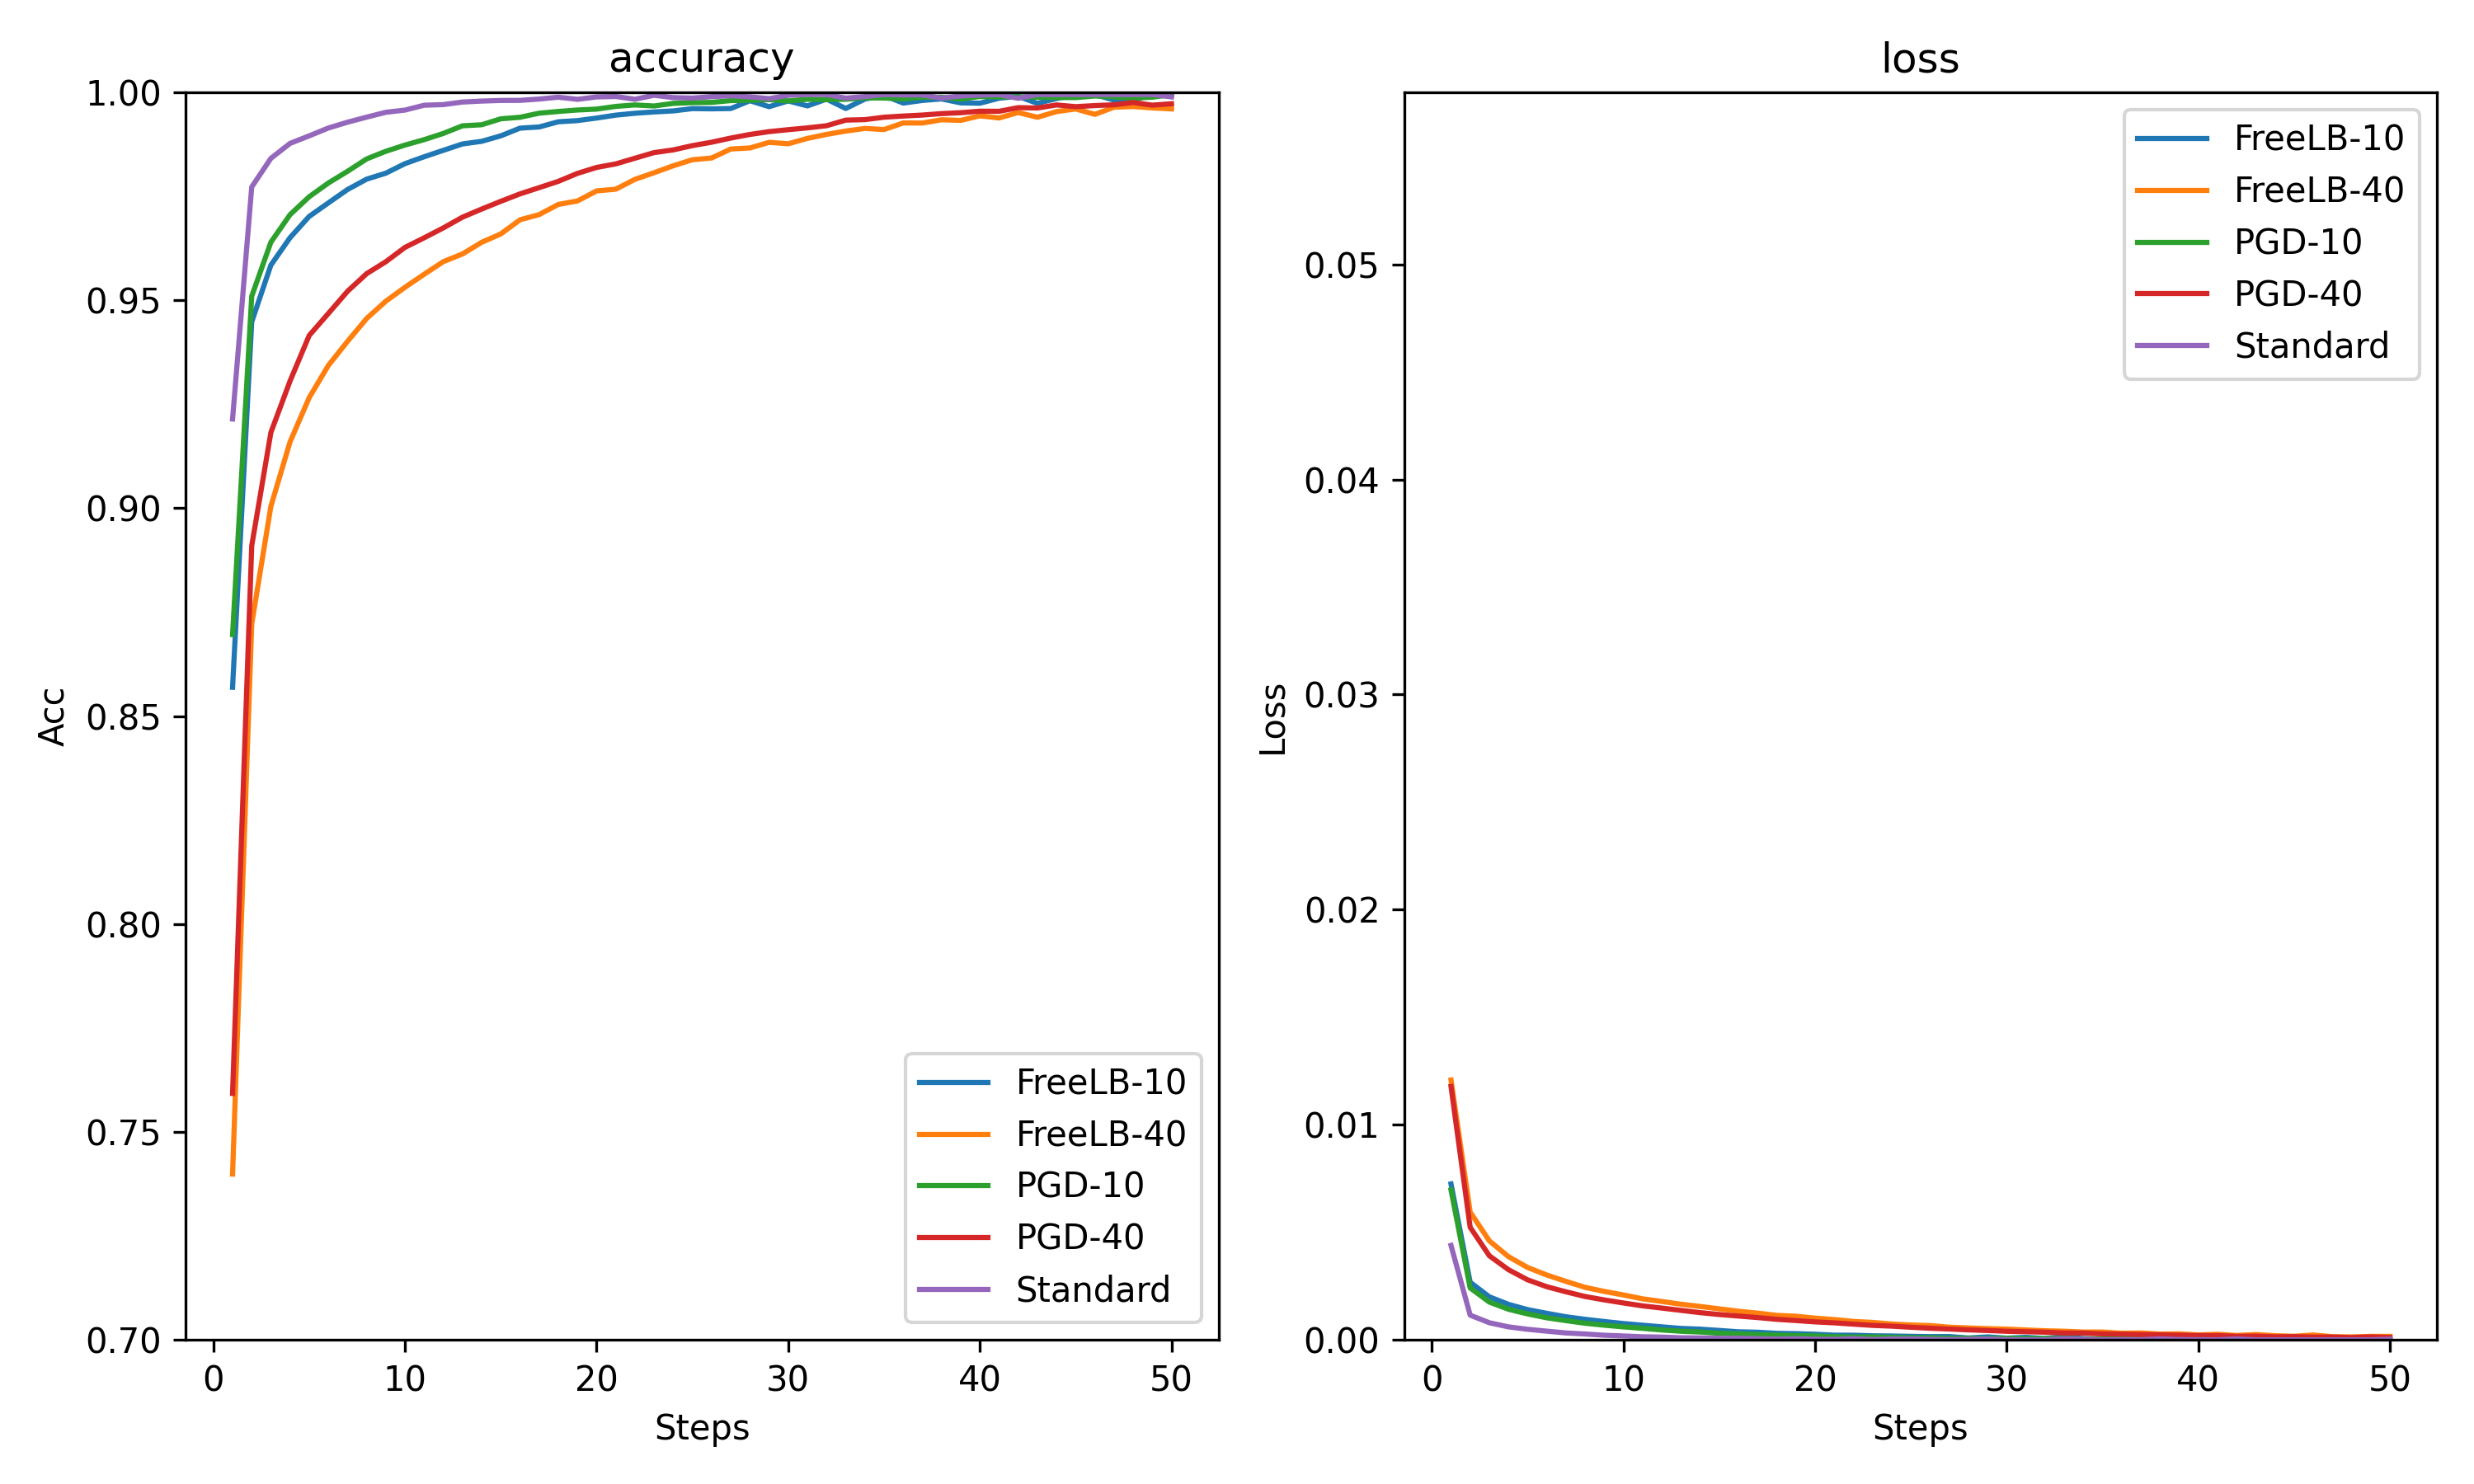
\includegraphics[width=0.45\textwidth]{figures/plot-Training.png}
\end{figure}


The results reveal several key insights into adversarial training:

First, models trained with adversarial examples tend to exhibit slightly reduced performance on clean (unperturbed) test data compared to those trained under standard conditions. This performance drop becomes more pronounced as the number of inner-loop adversarial iterations increases, which correlates with the intensity of the applied perturbations.

Second, adversarial training introduces significant computational overhead. As shown in Table~\ref{table:instance_training-result}, the training time increases considerably with the number of adversarial steps. This trade-off between robustness and training efficiency is an important consideration in practical deployment scenarios.

\section{Issues of Adversarial Training}
Although Adversarial Training (AT) is widely regarded as an effective approach to enhancing the robustness of neural networks, numerous studies have highlighted its significant limitations across various aspects.

\subsection{Generalization and Blind-Spot Attacks}
Zhang et al.~\cite{zhang2019limitationsadversarialtrainingblindspot} pointed out that AT shows considerably weaker robustness against samples located in low-density regions of the training data distribution. These so-called "blind-spot samples" lie far from the main data manifold and are often underrepresented during training, making them vulnerable to blind-spot attacks. This problem is particularly pronounced in high-dimensional datasets such as CIFAR-10 and ImageNet.

\subsection{Reliability Issues in Robot Learning}
Lechner et al.~\cite{lechner2021adversarialtrainingreadyrobot} demonstrated that AT can introduce new risks in robotic learning systems, including transient errors, systemic biases, and conditional failures. These issues suggest that in dynamic and complex environments, AT may compromise the model's stability and interpretability.

\subsection{High Computational Cost}
AT typically involves generating adversarial perturbations for each training example, such as using Projected Gradient Descent (PGD), which significantly increases training time and resource consumption. Zhao et al.~\cite{zhao2022review} noted that such overhead may become a bottleneck in real-world industrial deployments, especially in resource-constrained or latency-critical systems.

\subsection{Accuracy Degradation on Clean Samples}
Adversarial training often comes at the cost of reduced accuracy on clean (non-adversarial) inputs. Zhao et al.~\cite{a15080283} observed in their systematic review that this "robustness-accuracy trade-off" is a central challenge in current AT methods, and can be particularly problematic in domains where high accuracy is essential, such as medical diagnosis. The result of training instance on \cref{table:instance_training-result} indicates this issues by that the accuracy of comparison of standard training and PGD-40 training. 

In summary, although adversarial training has made significant progress in improving adversarial robustness, its limitations—such as weak generalization, high training overhead, and performance degradation on clean data—necessitate further research and refinement.

\section{Further Applications}

Adversarial training has proven to be a versatile framework beyond its original role in enhancing model robustness against malicious perturbations. In particular, it underpins two prominent domains: generative modeling—most notably Generative Adversarial Networks (GANs)—and adversarial explainability, which leverages adversarial perturbations to illuminate the decision-making processes of complex models.

\subsection{Generative Modeling via Adversarial Games}

In the context of generative modeling, adversarial training formulates a two-player minimax optimization between a \emph{generator} $G$ and a \emph{discriminator} $D$. Given a noise prior $z\sim p_z(z)$ and real data distribution $x\sim p_{\mathrm{data}}(x)$, the objective is

$$
\begin{aligned}
\min_{G} &\max_{D} V(D,G)= \\
& \mathbb{E}_{x\sim p_{\mathrm{data}}}\bigl[\log D(x)\bigr]
\;+\;\mathbb{E}_{z\sim p_z}\bigl[\log\bigl(1 - D(G(z))\bigr)\bigr]
\end{aligned}
$$

Here, $D$ aims to accurately distinguish genuine samples from synthetic ones $G(z)$, while $G$ seeks to generate data that aligns with the empirical distribution. At equilibrium, $G$ reproduces the data distribution and $D$ attains maximal entropy ($D(\cdot)=0.5$) \cite{goodfellow2014generativeadversarialnetworks}. Variants such as Wasserstein GANs (WGAN) and Deep Convolutional GANs (DCGAN) have been developed to improve optimization stability and sample fidelity.

\subsection{Adversarial Explainability}

Adversarial explainability uses perturbation analysis to explore model interpretability. For a classifier $f: \mathbb{R}^n\to{1,\dots,K}$ and input $x$, one determines the minimal perturbation $\delta$ that alters the predicted label:

$$
\begin{aligned}
\delta^* &= \arg\min_{\|\delta\|\le\epsilon} \|\delta\| \\
\text{s.t.}&\quad
\arg\max_x f(x+\delta) \neq \arg\max_x f(x)
\end{aligned}
$$

The vector $\delta^*$ highlights input dimensions critical to the decision boundary: components with larger magnitude indicate features to which $f$ is most responsive. Such perturbations can be visualized as sensitivity maps or quantified as feature importance scores, thereby elucidating the model's reliance on specific input characteristics \cite{NEURIPS2019_e2c420d9, tsipras2019robustnessoddsaccuracy}.

\medskip
In summary, adversarial training serves a dual purpose: as a generative mechanism producing high-quality synthetic samples, and as a diagnostic tool revealing the sensitivities of neural models. Its formulation as minimax optimization provides a unified theoretical foundation for both applications.

\section{Conclusion}

In this report, we have presented a comprehensive exploration of adversarial training, beginning from its theoretical underpinnings to practical algorithmic implementations. We formally defined the robust optimization objective and surveyed state-of-the-art methods including PGD-based training and FreeLB. Through a controlled empirical study on a lightweight convolutional neural network, we demonstrated that adversarial training markedly enhances model robustness—elevating accuracy under strong perturbations from approximately 56\% to over 95\%—while incurring only a modest reduction in clean-data performance. We also highlighted the substantial computational overhead introduced by multi-step adversarial methods, which poses a significant barrier to large-scale deployment.

Despite these challenges, adversarial training remains the most effective defense strategy against worst-case perturbations. Addressing its limitations requires future work in several directions: developing more efficient optimization schemes to reduce training time, designing adaptive perturbation strategies that balance robustness and accuracy, and extending adversarial frameworks to diverse modalities such as text and graph-structured data. Furthermore, deeper theoretical analyses are needed to understand the fundamental trade-offs between robustness, generalization, and computational complexity. By advancing both the practical and theoretical aspects of adversarial training, we can move closer to deploying machine learning models that are both high-performing and resilient in real-world, adversarial environments.

{\small
\bibliographystyle{ieeenat_fullname}
\bibliography{references}
}
\end{document}

